This talk was given by \emph{Danil}
The main reference is \cite{seidel2001vanishing,seidel2001more}.
\section{Fukaya Categories}
Let $(X, \omeg)$ be a $2n$ dimensional \ref{def:symplecticXanifold}. Fix an \ref{def_compatibleAlmostComplexStructure} $J$ on $X$. 

\begin{definition}[Novikov Field]
The \emph{Novikov field} with $\mathbb C$-coefficients is the ring of formal power series
\[\Lambda_{\geq 0}:=  \left\{\sum_{i=0}^\infty  a_i T^{\lambda_i}\st a_i\in \CC, \lambda \in \RR, \lim_{i\to\infty} \lambda_i = \infty\right\}.
\]
See also: \snip{the Novikov Ring}{def:novikovRing}
\end{definition}

\begin{definition}[Lagrangian Intersection Floer groups]
  Let $(X, \omega)$ be a symplectic manifold. Let $L_0, L_1\subset (X, \omega)$ be Lagrangian submanifolds whose intersection in $X$ is transverse. The \emph{Lagrangiain intersection Floer complex} is the vector space 
  \[\CF(L_0, L_1):= \bigoplus_{q\in L_0\cap L_1} \Lambda \langle p\rangle \]
  equipped with an endomorphism $\partial: \CF(L_0, L_1)\to \CF(L_0, L_1)$ whose structure coefficients are given by counts of psuedoholomorphic disks. For $p,q\in L_0\cap L_1$ and $\beta\in H_2(X, L_1\cup L_2, \ZZ)$, consider the moduli space of strips: 
  \[\mathcal M(p, q, \beta):= \left\{u: \RR\times [0, 1]\to X \middle | \begin{array}{cc} u(s, t)\to p & \text{ as } s\to-\infty \\ u(s, t)\to q & \text{ as } s\to \infty \\ u(s, 0) \in L_0, u(s, 1)\in L_1 \\ [u]=\beta \end{array}\right. / \RR\]
  We work over $\Lambda$ to ensure convergence of the differential.
\end{definition} 

Under some extra assumptions, $(m^1)^2=0$, so we get some well-defined cohomology groups $\HF(L_0, L_1)$, called the Lagrangian intersection Floer cohomology groups of $L_0, L_1$. 
\begin{theorem}[Invariance of Lagrangian intersection Floer cohomology]
Under appropriate conditions, the Lagrangian intersection Floer cohomology is independent of choices made in its definition and the Hamiltonian isotopy class of $L_0$ or $L_1$.
\end{theorem}
\begin{theorem}[PSS isomorphism]
If $L$ bounds no psuedoholomorphic disks, then $\HF(L, L)\simeq H^\bullet(L, \Lambda)$. 
\end{theorem}
\begin{definition}[Fukaya Category]
The Fukaya category $\Fuk(X)$ is an $\Lambda$-linear \snip{$A_\infty$ category}{def:aInfinityCategory} whose 
\begin{enumerate}
\item objects are mutually transverse \snip{Lagrangian submanifolds}{def:lagrangianSubmanifold} 
\item morphisms are generated by the Lagrangian Intersection Floer groups  $\CF(L_0, L_1 )$
\item compositions $m^2$ are given by counts of pseudoholomorphic triangles.
\end{enumerate}
We also have some higher maps $m^k: \hom(L_{k-1}, L_k)\tensor \cdots \hom(L_0, L_1)\to \hom(L_0, L_k)[2-k]$ given by counting holomorphic $k+1$-gons. 
\end{definition}
With extra assumptions on the symplectic manifold $X$ and Lagrangians $L$, we can equip $\Fuk(X)$ with a $\ZZ$-grading. 

\section{Fukaya categories in the non-compact setting}
%label:"def:liouvilleDomain"
%author:JeffHicks
%name:"Liouville domain"
%type:"definition"

 
    A Liouville domain is a pair $(X,\lambda)$, where
    \begin{itemize}
       \item $X$ is a $2n$-manifold with boundary $\partial X$ and,
       \item $\lambda\in \Omega^1(X, \RR)$ is a one form on $\Omega^1(X, \RR)$ so that $\omega=d\lambda$ is a symplectic form for $X$.
    \end{itemize}
 To this data we can associate a \emph{Liouville vector field} $Z$ defined by the property $\iota_Z\omega= \lambda$.
 We require that this vector field transversely points outward along $\partial X$.
 \label{def:liouvilleDomain}
 
%label:"def:symplecticCotangentBundle"
%type:"example"
%name:"symplectic structure on cotangent bundle"


    Let $Q$ be a smooth $n$-dimensional manifold.
    We now describe a canonical symplectic form on the cotangent bundle, $T^*Q$.
    At every point $q\in Q$, there exists chart $q\in U\subset Q$ which we can parameterize with coordinates $(q_1, \ldots, q_n)$.
    The cotangent bundle $T^*U$ inherits coordinates $(q_1, p_1, q_2, p_2, \ldots, q_n, p_n)$, where the $p_i$ linearly parameterize the fibers of the cotangent bundle in the direction of the basis element $dq_i$.
    \footnote{ The letter $p$ is chosen for historical reasons. The form $dq_i$ is dual to the vector $\partial q_i$, which represents the velocity of a particle.     The dual to velocity is momentum, which was historically represented by the variable $\rho$.    Therefore, the momentum coordinates have been denoted by $p_i$.  } 
    In these coordinates, the canonical symplectic form on this chart is:
    \[\omega=\sum_{i=1}^n dq_i \wedge dp_i=-d(p dq).\]


%tag:0007
%label:"exm:cotangentBundleIsLiouville"
%author:JeffHicks
%name:"Liouville structure on the cotangent bundle"
%type:"example"
%parent:def:liouvilleDomain


    Let $Q$ be a manifold. The cotangent bundle $X=T^*Q$ is an exact symplectic manifold; call the primitive $\lambda_{can}=\sum_{i=1}^np_idq_i$. In local coordinates, the Liouville vector field is $Z= \sum_{i=1}^n p_i \partial p_i$. The flow of this vector field acts by scalar multiplication on the fibers of $T^*Q$,
    \begin{align*}\phi^t: T^*Q\to T^*Q && (q, p) \mapsto (q, tp)\end{align*}
    which inflates the symplectic form.

    Now equip $Q$ with a metric $g$. The metric determines a unit sphere bundle $S^*Q\subset T^*Q$, which is transverse to $V$. Letting $\alpha=\lambda|_{S^*Q}$ makes  $(S^*Q, \alpha)$ a contact manifold. The time $t$-flow on  $(S^*Q, \alpha)$ corresponds to the time $t$ geodesic flow on the base (\cref{exr:geodesicsInSymplecticCohomology}). It is known (\cite{fet1952variational}) that every closed manifold has at least 1 closed geodesic, so all of these examples of contact manifolds have a Reeb orbit. 



\input{def_wrappedFukayaCategory}


\begin{example}[Wrapped Floer cohomology in cotangent bundle of the circle]
  \label{ex:wrappedFloerCohomology}
  To compute the wrapped Floer cohomlogy of $L:=T^*_0S^1\subset T^*S^1$ with itself, we first wrap the Lagrangian submanifold with the Hamiltonian $p^2: T^*S^1\to \RR$. This gives the red ``spiral'', $L^w$ drawn in the picture below. The intersections between $L, L^w$ are in bijection with the integers. After fixing an intersection point $(`` e'')$, we (suggestively) identify the Lagrangian intersection Floer cochains with the polynomial algebra. $\Hom(L, L)\simeq \CC[x, x^{-1}]$. 
  %label:"fig:wrappedFloerCylinder"
%author:JeffHicks
%name:"Floer theory of zero section in $T^*S^1$"
%type:"figure"
%parent:"exm:wrappedFloerCylinder"
%caption:"Computation of the wrapped Floer cohomology of the cotangent fiber with itself in $T^*S^1$."
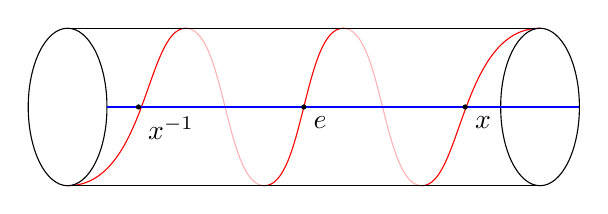
\begin{tikzpicture}
    \begin{scope}[]
    \draw[red] (-4,-0.5) .. controls (-3,-0.5) and (-3,1.5) .. (-2.5,1.5) .. controls (-2,1.5) and (-2,-0.5) .. (-1.5,-0.5) .. controls (-1,-0.5) and (-1,1.5) .. (-0.5,1.5) .. controls (0,1.5) and (0,-0.5) .. (0.5,-0.5) .. controls (1,-0.5) and (1,1.5) .. (2,1.5);
    \fill[white, opacity=.7]  (-2.5,1.5) rectangle (-1.5,-0.5);
    \fill[white, opacity=.7]  (-0.5,1.5) rectangle (0.5,-0.5);
    \end{scope}
    \draw  (-4,0.5) ellipse (0.5 and 1);
    \draw  (2,0.5) ellipse (0.5 and 1);
    \draw (-4,1.5) -- (2,1.5)  (-4,-0.5) -- (2,-0.5);
    \draw[blue] (-3.5,0.5) -- (2.5,0.5);
    
    \node[circle, fill=black, scale=.2] at (-3.1,0.5) {};
    \node[circle, fill=black, scale=.2] at (-1,0.5) {};
    \node[circle, fill=black, scale=.2] at (1.05,0.5) {};
    
    
    \node[below right] at (-3.1,0.5) {$x^{-1}$};
    \node[below right] at (-1,0.5) {$e$};
    \node[below right] at (1.05,0.5) {$x$};
\end{tikzpicture}
  In fact, this identification sends the Floer theoretic product (given by counts of holomorphic polygons) to the product structre on $\CC[x, x^{-1}]$. 
\end{example}

This provides us with a method for understanding the Fukaya category of a non-compact manifold; we will additionally want to incorporate the data of a potential so taht we can study the Fukaya category of a symplectic Landau-Ginzberg model. 
\section{Symplectic Fibrations}
\begin{definition}[exact symplectic fibration]
  \label{def:exactSymplecticFibration}
  Let $B$ be a symplectic manifold with boundary; for example $(B=D^2\subset \CC)$. 
  An \emph{exact symplectic fibration} is a smooth proper fiber bundle $\pi: E|to B$ such that:
  \begin{itemize}
  \item $E$ is a manifold with codimension two corners, and a decomposition of the boundary into a vertical and horizontal component $\partial E= \partial_h E\cup \partial_v E$;
  \item We have differential forms $\omega\in \Omega^2(E), \theta\in \Omega^1(E)$ such that $E_z=\pi^{-1}(z)$ is a Liouville domain with symplectic form $\omega_z=\omega|_{E_z}$ whose primitive $\theta_z=\theta|_{E_z}$;
  \item The fibration $\pi$ is ``trivial'' near the horizontal boundary.
  \end{itemize}
\end{definition}
\begin{definition}[exact Landau-Ginzberg model]
\label{def:exactLGModel}
An \emph{exact LG model} is an exact symplectic manifold $(E, \omega=d\theta)$ that carries a proper smooth map $\pi: E\to D^2$ with a compatible almost complex structure $J$ making $\pi$ holomorphic. Furthermore, we require the locus of critical points $\Crit(\pi)$ to be disjoint from $\partial_h E$ and $\pi$ is a exact symplectic fibration away from the $\Crit(\pi)$. 
\end{definition}
\begin{definition}[Lefschetz fibration]
  \label{def:lefschetzFibration}
We will call a \snip{exact LG model}{def:exactLGModel} $(E, \pi)$ a \emph{Lefschetz fibration} if $\Crit(\pi)$ is a fibite set of points, every fiber has at most one critical point, and $\pi$ is ``Morse'' in the sense that it is locally modelled on the fibration $\pi(z_1, \ldots, z_n)= z_1^1+\cdots + z_n^2$. 
\end{definition}
\begin{example}[my first Lefschetz fibration]
Let $B=D^2\susbet \CC$, let $E=left\{ z\in \CC^n \st \left|\sum_{i=1}^n z_i^2\right|\leq 1, \|z\|\leq Tright\}$ for some $T>1$, then we have a Lefschetz fibration 
\begin{align*}
\pi: E\to &B\\
z\mapsto & z_1^2+\cdots + z_n^2
\end{align*}
\end{example}
\begin{example}[a non-Lefschetz fibration]
  Consider the map 
  \begin{align*}
  \CC^3\to & \CC\\
  (x, y, z) \mapsto & xyz.
  \end{align*}
  This is an example mirror to the pair-of-pants.
\end{example}
\begin{example}[Lefschetz fibration from a pencil]
Given a smooth projective variety $X$, an ample line bundle $L\to X$, pick two sections $\sigma_0, \sigma_1\in H^0(L)$ to give a Lefschetz pencil. From the data of a Lefschetz pencil we can define an exact Lefschetz fibration 
\[E:=X\setminus Y_\infty, \pi(x)=\frac{\sigma_0(x)}{\sigma_1(z)}\]
where $Y_t=\{x\in X \st \sigma_1(x)/\sigma_0(x)=z\}$, 
Then $\pi: E\to \CC$ is a Lefschetz fibration. 
\end{example}
\begin{theorem}
  The Lagrangian intersection Floer cohomology of a pair of Lagrangian thimbles
  $L_i, L_j$ in a Lefschetz fibration,
  can be computed in the fiber as 
  \[\hom_{\FS(Y, W)}(L_i, L_j)= \left\{\begin{array}{cc}\hom_{\Fuk(Y_t)}(V_i, V_j) & \text{ if } i<j \\
    \CC\cdot x_i & \text{ if } i=j\\
    0 & \text{ if } i>j
  \end{array}\right.
  \]
\end{theorem}
%source:Seidel
\begin{corollary}
  The Lagrangian $\langle L_1, \ldots, L_k\rangle$ form a full exceptional collection. 
\end{corollary}

\section{Exceptional collections from a mutation}
Here, fix a Lefschetz fibration $W: Y\to \CC$ with critical values $\lambda_1, \ldots, \lambda_k\in \CC$. Pick a collection of \snap{vanishing paths}{def:vanishingPaths} for the $\lambda_j$. This gives us Lagrangian thimbles $L_1, \cdots, L_k$, and vanishing cycles $V_1, \ldots, V_k$ (which are Lagrangians inside some fixed fiber $W^{-1}(t)$, where $t\gg 0$. )
\section{Mutations}
We now have a full exceptional collections. We can modify a set of vanishing paths by ``twisting'' them in the base of the Lefschetz fibration.

\begin{figure}
%name:mutation of vanishing paths
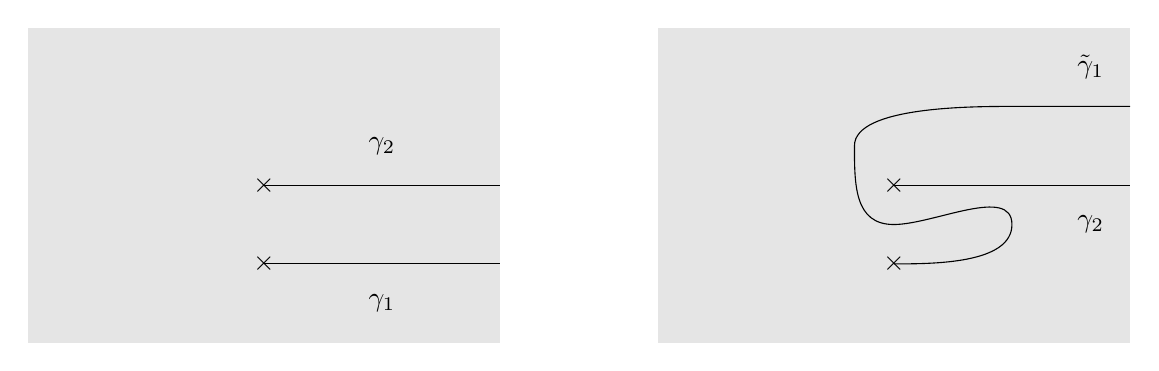
\begin{tikzpicture}

  \begin{scope}[]
  \fill[gray!20] (8,2.5) rectangle (2,-1.5);
  \node at (5,-0.5) {$\times$};
  \node at (5,0.5) {$\times$};
  \draw (5,-0.5) -- (8,-0.5) ;
  \draw (5,0.5) -- (8,0.5);
  \node at (6.5,-1) {$\gamma_1$};
  \node at (6.5,1) {$\gamma_2$};
  \end{scope}
  \begin{scope}[shift={(8,0)}]
  \fill[gray!20] (8,2.5) rectangle (2,-1.5);
  \node at (5,-0.5) {$\times$};
  \node at (5,0.5) {$\times$};
  \draw (5,0.5) -- (8,0.5);
  \node at (7.5,2) {$\tilde\gamma_1$};
  \node at (7.5,0) {$\gamma_2$};
  \end{scope}
  \draw (13,-0.5) .. controls (13.5,-0.5) and (14.5,-0.5) .. (14.5,0) .. controls (14.5,0.5) and (13.5,0) .. (13,0) .. controls (12.5,0) and (12.5,0.5) .. (12.5,1) .. controls (12.5,1.5) and (14,1.5) .. (14.5,1.5) .. controls (15,1.5) and (15.5,1.5) .. (16,1.5);
  \end{tikzpicture}
  \caption{We can mutate vanishing cycles in the base of a LG fibration}
\end{figure}




@inproceedings{seidel2001vanishing,
  title={Vanishing cycles and mutation},
  author={Seidel, Paul},
  booktitle={European Congress of Xathematics: Barcelona, July 10--14, 2000 Volume II},
  pages={65--85},
  year={2001},
  organization={Springer}
}

@article{seidel2001more,
  title={More about vanishing cycles and mutation},
  author={Seidel, Paul},
  journal={Symplectic geometry and mirror symmetry (Seoul, 2000)},
  pages={429--465},
  year={2001}
}